\documentclass[10pt]{beamer}

\usetheme{metropolis}
\usepackage{appendixnumberbeamer}

\usepackage{booktabs}
\usepackage[scale=2]{ccicons}
\usepackage{pgfplots}
\usepgfplotslibrary{dateplot}

\usepackage{xspace}
\newcommand{\themename}{\textbf{\textsc{metropolis}}\xspace}

\title{Machine Learning and QCD}
\subtitle{for Proton structure determination}
\date{January, 2020}
\author{Alessandro Candido - Roy Stegeman \\
{\footnotesize supervisor:} Stefano Forte, Stefano Carrazza
}
%\institute{N3PDF}
\titlegraphic{\hfill
		\raisebox{5pt}[0pt][0pt]{
\includegraphics[height=0.8cm]{n3pdf_logo.png}}\hspace*{10pt}
		
\includegraphics[height=1.1cm]{erc_logo.png}
		
		\vfill\vspace*{170pt}
		
\includegraphics[height=1cm]{unimi_logo.png}\hfill
		
\includegraphics[height=1cm]{infn_logo.png}
	}

\begin{document}

\maketitle

\begin{frame}{Theory}

Parton Distribution Functions (PDF) describe the internal structure of the proton, as it is made by its constituents.
\vspace*{10pt}

\begin{columns}[T,onlytextwidth]
	\column{0.45\textwidth}
	\begin{itemize}
		\item PDFs are determined from the experimental data (\textit{fit})
%		QCD is non-perturbative at the proton scale, and in the UV there is no proton around
		\item they are used to make theoretical predictions for collider observables (\textit{factorization})
%		\item the theoretical knowledge is used to make a proper fit 
		\item the goal is to improve the accuracy of PDFs and their features (e.g.: \textit{NLO positivity})
	\end{itemize}
	\column{0.05\textwidth}
	\column{0.5\textwidth}
	\vspace*{20pt}
	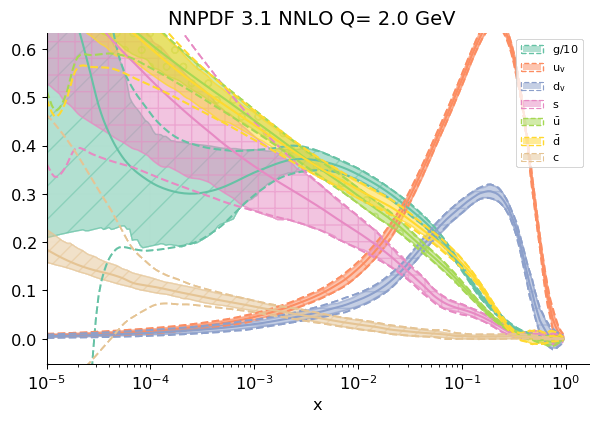
\includegraphics[width=0.95\textwidth]{nnpdf31_}
\end{columns}

\end{frame}

\begin{frame}{Machine Learning}

\end{frame}

\end{document}
